%\documentclass[11pt]{scrartcl}
\documentclass[11pt]{article}
\usepackage[utf8]{inputenc}
\usepackage{cmap}
\usepackage[T1]{fontenc}
\usepackage{lmodern}
\usepackage[brazil]{babel}

%\usepackage{lrsmath}
\usepackage{url}
\usepackage{enumerate}
\usepackage{indentfirst}
\usepackage{acronym}

\usepackage{amsmath}
\usepackage{booktabs}
\usepackage{amssymb}
\usepackage{amsthm}
\usepackage{amscd}
\usepackage{amsfonts}
\usepackage{dsfont}
\usepackage{color}
\usepackage{multicol}

\usepackage[table]{xcolor}

\usepackage{graphicx}
\usepackage{tikz}
\usetikzlibrary{arrows,shapes,positioning,shadows,trees}


\tikzset{
  basic/.style  = {draw, text width=2cm, drop shadow, font=\sffamily, rectangle},
  root/.style = {basic, rounded corners=6pt, thin,align=center, fill=green!30,
                   text width=8em},
  level 2/.style = {basic, rounded corners=6pt, thin,align=center, fill=green!30,
                   text width=8em,sibling distance=10mm}
  level 3/.style = {basic, rounded corners=2pt, thin,align=center, fill=green!30,
                    innersep = 10mm,sibling distance=10mm}
}

\usepackage{graphicx}

\usepackage{3dplot}

\newtheorem{defi}{Definição}[section]
\newtheorem{teo}{Teorema}[section]
\newtheorem{cor}{Corolário}[section]
\newtheorem{conj}{Conjectura}[section]
\newtheorem*{propri}{Propriedades}
\newtheorem{pro}{Proposição}[section]
\newtheorem{lema}{Lema}[section]
\newtheorem{obs}{Observação}[section]
\newtheorem{ex}{Exemplo}[section]

\newtheorem*{DGP}{{\emph{Distance Geometry Problem (DGP)}}}

\newtheorem*{iMDGP}{{\emph{interval Molecular Distance Geometry Problem (iMDGP)}}}

\newtheorem*{MDGP}{{\emph{Molecular Distance Geometry Problem (MDGP)}}}

\newtheorem*{DMDGP}{{\emph{Discretizable Molecular Distance Geometry Problem (DMDGP)}}}

\newtheorem*{DDGP}{{\emph{Discretizable Distance Geometry Problem $k =3$ (DDGP$_3$)}}}

\newtheorem*{DVOP}{{\emph{Discretization Vertex Order Problem (DVOP)}}}

\usepackage[top=3cm,bottom=3cm,right=2.5cm,left=2.5cm]{geometry}

%\usepackage[backend=biber,style=numeric-comp]{biblatex}
%\usepackage{csquotes}
%\addbibresource{references_bibdesk_papers.bib}

% \usepackage{showlabels} 

\usepackage{geometry}
\geometry{a4paper,top=3cm,left=2.5cm,right=2.5cm}



%\def\Dew{\Delta w}
%\def\Dex{\Delta x}
%\def\Dey{\Delta y}
%\def\Dez{\Delta z}
%\def\Cset{\mathcal{C}}

\begin{document}

%\title{Projeto de Pesquisa}
%\author{Projeto de Atividades Acadêmicas  \\ \textsc{Felipe Delfini Caetano Fidalgo}\thanks{\tt{felipaomat@gmail.com}}}
%\date{Maio de 2015}  
%\thispagestyle{empty}
%
%\maketitle

\begin{titlepage}

\newcommand{\HRule}{\rule{\linewidth}{0.5mm}} % Defines a new command for the horizontal lines, change thickness here

\center % Center everything on the page
 
%----------------------------------------------------------------------------------------
%	HEADING SECTIONS
%----------------------------------------------------------------------------------------

\begin{center}

\includegraphics[scale=0.22]{logoufsc}
\end{center}

\vspace{1cm}

\textsc{\LARGE Universidade Federal de Santa Catarina}\\[0.5cm] % Name of your university/college
{\Large Centro de Blumenau \\ Departamento de Matemática}\\[1.5cm] % Major heading such as course name
\textsc{\Large PIBIC \\ Programa Institucional de Bolsas de Iniciação Científica \vspace{1.5cm} \\ {ÁREA: Matemática}}\\[2.0cm] % Minor heading such as course title

%\textsc{\LARGE Universidade Federal de Santa Catarina}\\[0.5cm] % Name of your university/college
%{\Large Centro de Blumenau \\ Departamento de Matemática}\\[1.5cm] % Major heading such as course name
%\textsc{\Large PIBIC \\ Programa Institucional de Bolsas de Iniciação Científica \vspace{1.5cm} \\ {\bf PROJETO DE PESQUISA}}\\[2.0cm] % Minor heading such as course title

%----------------------------------------------------------------------------------------
%	TITLE SECTION
%----------------------------------------------------------------------------------------

\HRule \\[0.4cm]
{ \LARGE \bfseries Disposição de Robôs Móveis no espaço Euclidiano 3D: uma aplicação de Geometria de Distâncias} \\ [0.4cm] % Title of your document
\HRule \\[2.5cm]
 
%----------------------------------------------------------------------------------------
%	AUTHOR SECTION
%----------------------------------------------------------------------------------------

\begin{minipage}{0.4\textwidth}
\begin{center} \large
\underline{\textsc{Orientador:}} \vspace{0.2cm} \\
Dr. Felipe Delfini Caetano Fidalgo 
\end{center}
\end{minipage} \\[2cm]


{\large \today} % Date, change the \today to a set date if you want to be precise


\vfill % Fill the rest of the page with whitespace

\end{titlepage}

\tableofcontents


\section{Resumo}

O tema deste projeto é estudar uma forma de obter as localizações de entidades móveis independentes (Robôs Móveis) que compõem um sistema autônomo, através da aplicação de Geometria de Distâncias na descoberta por conformações tridimensionais válidas. Saber esta estrutura tridimensional é um passo importantíssimo para a organização e realização das tarefas dessas entidades.

O principal problema envolvido é o DDGP ({\emph{Discretizable Distance Geometry Problem}}), do inglês, Problema de Geometria de Distâncias Discretizáveis, cuja ferramenta de solução numérica é dada pelo Algoritmo Branch-and-Prune (BP). 

Este algorítimo tem por base o fato de discretizarmos o número de soluções possíveis do problema. A ideia central por trás dessa discretização vem de que, no geral, a intersecção de $K$ esferas em um espaço $\mathbb{R}^K$ determina, no máximo, dois pontos. Porém, para conseguirmos tal discretização, surge outro problema, conhecido como DVOP (\emph{Discretizable Vertex Order Problem}), isto é, o problema de encontrar uma ordem nos vértices tal que sempre consigamos a intersecção de $K$ esferas. \cite{carlile:DDGP}

O projeto requer um aluno bolsista que deve estudar a motivação (Sistemas de Robôs Móveis), o DDGP, o DVOP, o Algoritmo BP e, por fim, realizar experimentos computacionais com o objetivo de realizações práticas do estudo.

\begin{obs}
	Este projeto está vinculado, como subprojeto, ao projeto de pesquisa docente ``Geometria de Distâncias e Álgebras Geométricas: novas perspectivas geométricas, computacionais e aplicações'', registrado no SIGPEX sob o número 201801170, devidamente aprovado no departamento.
\end{obs}


\section{Introdução}

A Geometria de Distâncias (GD) é uma matéria de interesse relativamente recente da Ciência, disposta em uma vasta interseção entre diversas áreas do conhecimento. Em suma, ela se preocupa com os aspectos geométricos decorrentes dos objetos que estão dispostos em algum espaço e possuem entre si uma relação de distância, podendo esta ser considerada da maneira mais abrangente possível (duas obras do matemático franco-soviético Michel Marie Deza {\emph{et al.}} fornecem uma ampla gama de distâncias, bem como suas possíveis aplicações:  {\emph{Dictionary of Distances}} \cite{deza2006dictionary} e {\emph{Encyclopedia of Distances}} \cite{deza2009encyclopedia}).

O problema principal a ser discutido no trabalho que é objeto deste projeto será uma particularização do chamado {\emph{Distance Geometry Problem}} (DGP) (ou, Problema de Geometria de Distâncias) monido de uma ordem para seus vértices tal qual permita que seja discretizado, para que se possa localizar objetos no espaço.

Apresentamos, a seguir, a motivação e a contextualização teórica do projeto.


\subsection{Motivação: Solução para Problemas Reais}	
Quando se apresenta um problema onde se deve organizar peças móveis em um sistema, sabendo que esta organização está intrinsecamente ligada a controlar suas localizações precisas, logo surgem propostas de soluções muito bem conhecidas para obter-se estas localizações, como utilizar o sistemas de posicionamento global (GPS) ou derivados em menor escala (em suma, trilateração hiperbólica). Porém, tais soluções costumam ser custosas \cite{savvides2001dynamic}, necessitando de alguns pontos distribuídos de forma esperta no espaço do problema para serem utilizados como ancora em relação aos demais pontos a serem localizados (como os satélites no caso do GPS), ou seja, propõe-se que todas as localizações sejam dadas medindo-se distâncias a pontos ancorados, isto é, com localização bem definida.

O objetivo desse trabalho é propor um paradigma diferente na obtenção dessas localizações. Ao invés de usarmos distâncias em relação a pontos fixos para obtermos realizações dos objetos no espaço cartesiano, sugere-se a utilização de um novo sistema de coordenadas onde os dados são medidos sempre entre os próprios pontos do sistema, independentes de pontos previamente localizados, e, através da geometria de distâncias, estima-se as coordenadas cartesianas destes pontos no espaço tridimensional em relação a eles mesmos. Essas posições são de grande importância para que objetos autônomos consigam se organizar em um espaço.

Vemos uma tendencia de mercado em se adotar sistemas autônomos para realizar funções que dependem de um grande número de maquinas, como o controle do estoque em um armazém, um sistema de entregas utilizando veículos aéreos não tripulados ou o cultivo e tratamento de grandes áreas de plantio. Veremos cada uma dessas maquinas autônomas envolvidas como vértices no sistema. Para estudar melhor a estrutura tridimensional formada por este conjunto de vértices, define-se como uma \textbf{Conformação} de um sistema à disposição instantânea de seus elementos no espaço 3D.

Note que estamos interessados em obter a conformação do sistema. Uma mesma conformação pode ser representada no espaço cartesiano de infinitas formas diferentes, aplicando-se rotações e translações a estrutura. Caso seja parte do objetivo da aplicação, e no geral é, descobrir a localização dos robôs móveis em relação a outras entidades físicas do sistema (como as caixas em um armazém), pode-se tomar essas entidades também como parte da conformação, porém, definindo-as como ancoras.

\subsection{Obtenção de Dados}
Como se quer descobrir localizações, faz sentido que pensemos em um sistema que meça distâncias, pois é disso que se trata as coordenadas cartesianas. A coordenada $(x, y, z)$ de um ponto cartesiano diz as distâncias unidimensionais $x$, $y$ e $z$ de cada dimensão do espaço do problema ao ponto de origem, localizado na posição $(0, 0, 0)$. 

Porém, como estamos atrás de conformações, não nos ajuda inicialmente tratar sobre uma origem, pois tudo que temos quando olhamos para dois nós do sistema ($a$ e $b$) é sua distância $d(a,b)$. Quando temos três nós (ou seja, mais um nó $c$), só nos faz sentido as três distâncias $d(a,b)$, $d(a,c)$ e $d(b,c)$ e o angulo plano formado pelos três nós, no caso chamaremos de $\theta(a,c)$. Note que com essas quatro informações (se $a$, $b$ e $c$ não são colineares) formamos um triangulo e podemos localizar estes pontos no plano, porém temos infinitas possibilidades para suas posições devido possíveis rotações e translações desse triangulo. A mesma linha de raciocínio se mantém quando adicionamos mais um nó $d$ ao sistema, porém, aqui, temos um novo tipo de ângulo, chamado de ângulo de torção $\omega(a,d)$.

Como essas são as informações que podemos obter entre os nós dados do sistema, temos de utilizar um sistema de coordenadas condizente. Essas informações são muito bem descritas utilizando o chamado \textit{Sistema de Coordenadas Internas}.

\subsubsection{Sistema de Coordenadas Internas}

As coordenadas internas são definidas pela distância entre nós $d_{1,2}, ..., d_{n - 1,n}$, pelos ângulos planos $\theta_{1,3}, ...,\theta_{n - 2,n}$ (formados por 3 nós consecutivos) e pelos ângulos de torção $\omega_{1,4}, ..., \omega_{n-3,n}$ (formado por 4 nós consecutivos). O ângulo de torção se dá entre os planos formados pelos nós $i-3,i-2,i-1$ e$i-2,i-1,i$, respectivamente. Assim, temos que $\omega$ varia no intervalo $[0,2\pi]$ e $\theta$ de $[0,\pi]$, assemelhando-se ao sistema de coordenadas esféricas. Vide Figura ~\ref{fig:angulos}.
\\

\begin{figure}[h!]
	\begin{center}
		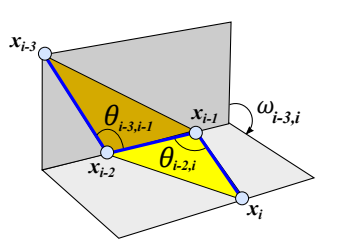
\includegraphics[width=0.5\linewidth]{cooint.png}
	\end{center}
	\caption{Coordenadas Internas}
	\label{fig:angulos}
\end{figure}

Mas ainda precisamos estudar uma forma de obter estas distâncias e ângulos. Pode-se obter os ângulos planos pela \textit{Lei dos Cossenos}, tendo em vista que conhece-se todas as distâncias que, por construção, representam os lados do triângulo. Também não se encontra dificuldades para determinar os ângulos de torção, podendo utilizar da \textit{Geometria Analítica} para descobrir o ângulo entre dois vetores e, lembrando, podemos representar um plano pelo vetor normal ao ele mesmo.

A dificuldade aqui está em obter as distâncias $d_{1,2}, ..., d_{n - 1,n}$. Para isso podemos utilizar métodos diferentes para cada tipo de aplicação, como, por exemplo, utilizar comunicação eletromagnética e medir o decaimento da força do sinal recebido (sabendo que a potência do sinal $P_{RSSI} = \frac{X}{R^n}$, onde $R$ é a distância percorrida pela onda eletromagnética). Também podemos utilizar métodos baseados no tempo, onde enviamos uma um sinal com velocidade conhecida e medimos o tempo que demora para esse sinal chegar ao destino, ou melhor, podemos enviar dois sinais no mesmo instante, com velocidades diferentes e conhecidas, para que possamos medir a diferença de tempo que as duas precisam para chegar ao outro nó e assim definir sua distância. Note a Figura ~\ref{fig:TDoA} que esboça isso com um sinal de radio em conjunto com um pulso de ultra-som.

\begin{figure}[h!]
	\begin{center}
		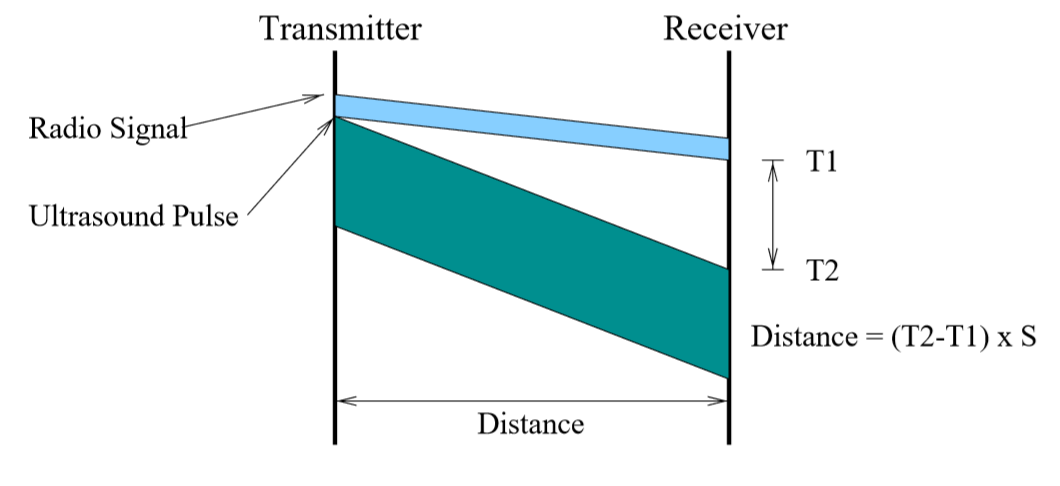
\includegraphics[width=0.8\linewidth]{TDoA.png}
	\end{center}
	\caption{Diferença entre sinais com velocidades conhecidas.}
	\label{fig:TDoA}
\end{figure}

\subsection{Contextualização: Geometria de Distâncias}

Este assunto emergiu, com relevância teórica, a partir de {\emph{Theory and Applications of Distance Geometry}} (1953) \cite{Blumenthal:53}, de L. M. Blumenthal. Baseando-se nos trabalhos pioneiros de Cayley \cite{Cayley:1841} e de Menger \cite{Menger:31}, ele desenvolveu o chamado Determinante de Cayley-Menger como ferramenta pra resolver ao problema fundamental a ser estudado, formulado como o seguinte problema de decisão: as entradas reais de uma dada matriz simétrica, de fato, consistem em distâncias entre pontos de um espaço Euclidiano? \cite{Survey:12}

Entretanto, a primeira referência explícita sobre o conceito contemporâneo do DGP foi dada por Y. Yemini em 1978, referindo-se a ele como {\emph{Positioning Problem}} (ou, Problema do Posicionamento). Em 1979, Yemini publicou outro artigo flexibilizando esta definição ao considerar dados de distâncias esparsas. Neste contexto, introduziu-se o {\emph{Problema Posição - Localização}, para o qual deseja-se calcular a localização de todos os objetos no espaço geográfico no qual estão inseridos \cite{Yemini:79,Survey:12}. Além disso, o autor faz uma análise de complexidade computacional para alguns problemas de rigidez em grafos, ferramenta que se tornara indispensável na modelagem dos problemas relativos a distâncias \cite{Survey:12}.
	
Ainda em 1979, J. Saxe publicou um trabalho lidando com aspectos análogos, sobre a imersão de um grafo em um espaço Euclidiano \cite{Saxe:79}, referindo-se ao DGP como ``{\emph{$K$ - Embeddability Problem}}'' (ou, K - Problema da Imersão) e demonstrando que: se o espaço é $\mathbb{R}$, este problema é {\bf NP} - Completo, caso contrário, ele é {\bf NP} - Difícil \cite{Survey:12}.

Em resumo, um DGP pertence à classe de problemas inversos, nos quais estamos interessados em fornecer uma distribuição de objetos, respeitando restrições de distâncias e simetria, intrínsecas ou fornecidas como entradas do problema \cite{Havel:95}.

Classicamente, o DGP é modelado e resolvido com a utilização recursos de Otimização Global Não-Linear:

\begin{equation}
\min \displaystyle \sum_{\{u,v\} \in E} \left( \left\| x_{u} - x_{v} \right\|^{2} - d^{2}_{uv} \right)^{2},  \label{eq:DGPpmform}
\end{equation}
onde $E$ é um conjunto de pares não-ordenados $\{ u,v \}$ para os quais se possui o valor de distância entre os pontos $u$ e $v$.

Um dos inconvenientes dessa abordagem e, portanto, dos respectivos métodos matemáticos-computacionais, é que este tipo de função, em geral, possui uma grande quantidade de mínimos locais, o que pode inviabilizar esta busca. Esta situação ainda é complicada pelo fato de que a quantidade de mínimos locais cresce exponencialmente em função do tamanho do problema. \cite{Survey:12,LavorCNMAC:14}. Por essas razões, passaram a buscar por modelos e soluções alternativos.

O DGP passa, então, a ser caracterizado através de Grafos \cite{Survey:12}, procurando-se imersões isométricas de um grafo que represente a instância em um espaço Euclidiano:

\begin{center}
	\begin{minipage}{0.9 \linewidth}
		\begin{DGP}
			Dado $K \in \mathbb{Z}_{+}$ e um grafo simples e não-direcionado $G = (V,E)$ cujas arestas são ponderadas pelos valores da função não-negativa $d: E \longrightarrow \mathbb{R}_{+}$, existem imersões $x:V \longrightarrow \mathbb{R}^{K}$ (realizações do grafo) tais que
			\begin{equation}
			\forall \{u,v\} \in E, \hspace{0.5cm} \left\| x_{u} - x_{v} \right\| = d_{u,v}? \label{eq:DGPdef}
			\end{equation}
		\end{DGP}
	\end{minipage}
\end{center}

Uma das ``belezas'' desse problema inverso é a ampla gama de possibilidades de se envolver em alguma aplicação em alguma outra área do conhecimento. Dessa feita, listamos algumas onde já se desenvolvem estudos com o DGP: Astronomia, Estática, Estatística, Estruturas Geométricas, Psicologia, Reconhecimento de Padrões, Redes de Computadores, Robótica, Códigos, Grafos, Visualização de Dados, Clustering, Data Mining, dentre outras. E a principal, por seu caráter pioneiro, tange o problema de encontrar conformações tridimensionais para estruturas moleculares.

A simples utilização de distâncias entre átomos e de quiralidade (simetria) auxiliou na precisa formulação matemática do problema de determinar a estrutura geométrica de moléculas, bem como de novas idéias e métodos eficientes para resolvê-lo. Assim, G. M. Crippen foi o pioneiro em utilizar GD para calcular conformações de estruturas moleculares, adaptando as idéias desenvolvidas por Blumenthal em {\emph{A Novel Approach to Calculation of Conformation: Distance Geometry}} (1977) \cite{Crippen:77}.

Logo, o problema que trata este documento pode ser encarado como uma particularização do DGP para $K = 3$. Esta particularização é denominada {\emph{Molecular Distance Geometry Problem}} (MDGP) - ou Problema de Geometria de Distâncias Moleculares \cite{LavorCNMAC:14}. Note que nosso problema não tem um suporte molecular, porém, devido a semelhança como os dois problemas são formulados e resolvidos, os dois se encaixam na mesma nomenclatura \cite{Survey:12} (neste trabalho há uma taxonomia da nomenclatura dos problemas da área). Na prática, o sistema de equações não lineares do MDGP não é resolvido por métodos exatos, mas de maneira aproximada considerando $| \left\|x_{i}-x_{j}\right\| -  d_{ij} |  < \varepsilon,$ onde o  erro $\varepsilon$ é definido de acordo com a aplicação.

\subsubsection{Descrição do Problema Fundamental}
Nesta seção, descrevemos o problema objeto deste projeto. Em seguida, vamos resumir as duas ferramentas a serem unidas a fim de aplicação para a resolução deste.

No geral, o conjunto solução para um DGP na terceira dimensão (não vazio) pode ser não enumerável ou finito \cite{carlileBook31Coloquio}. No caso finito, podemos explorar a estrutura do grafo que representa o problema para estudar novos métodos de solução. Dado um grafo $G = (V, E, d)$, quando queremos descobrir a posição de um vértice $s \in V$ no $\mathbb{R}^3$, duas informações são cruciais:
\begin{itemize}
	\item Existem $u, v, r \in V$ tais que $\{\{u,s\},\{v,s\},\{r,s\}\} \subset E$,
	\item $x_u, x_v, x_r \in \mathbb{R}^3$ fazem parte de uma realização ``parcial'' válida.
\end{itemize}

Essas duas informações estão relacionadas intrinsecamente com o conceito de \textit{ordem nos vértices} do grafo $G$ do DGP \cite{carlile:DDGP}. Isto é, podemos conseguir uma certa ordem no conjunto $V$ de tal forma que possamos garantir, a menos de rotações e translações, que o problema tem um conjunto solução enumerável e finito (de fato, um subconjunto finito do $\mathbb{R}^{3|V|}$). \cite{carlileBook31Coloquio}

Encontrar uma ordem para garantir a finitude do conjunto solução do problema, no geral, não é trivial e depende muito da natureza do problema. Encontrar essa ordem trata-se do $\emph{Problema da Ordem de Vértices Discretizáveis}$, ou simplesmente DVOP (do inglês, Discretization Vertex Order Problem). Segue sua definição formal:

\begin{DVOP}
	Dado um grafo simples não direcionado $G = (V, E)$ e um escalar positivo $K$, estabelecer se existe uma ordem < em $V$ tal que: 
	\begin{enumerate}
		\item[(a)] o subconjunto $\{v \in V \mid \rho(<,v) \leq K\} \subset V$ é um $K$-clique em $G$, e
		\item[(b)] para todo $v \in V$ com posto $\rho(<,v) > K$, temos $|\delta(v) \cap \gamma(<,v)| \geq K$.
	\end{enumerate}
Onde $\delta(v) = \{u \in V \mid  \{u,v\} \in E\}$; para a ordem < em $V$, tem-se $\gamma(<,v) = \{u \in V \mid u < v\}$ o conjunto de predecessores de $v$ na ordem < e $\rho(<,v) = |\gamma(v)| + 1$ o posto de v em < (a ordem é total porque V é finito).
\end{DVOP}

Supondo que existe uma ordem dada pela solução do DVOP no contexto do nosso problema, podemos definir formalmente o DDGP para a terceira dimensão, como segue.

\begin{DDGP} \label{def:DDGP}
	Dado um grafo ponderado e não-direcionado $G = (V,E,d)$, onde $d: E \longrightarrow \mathbb{R}_{+}$, o subconjunto de vértices $U_{0} = \{v_{1},v_{2},v_{3} \}$ e uma relação de ordem total em $V$ que satisfaz a seguinte relação de axiomas:
	\begin{enumerate}[(1)]
		\item $G[U_{0}]$ é um clique em três vértices (iniciando a configuração);
		\item para todo vértice $v_{i}$ com posto $i = \rho(v_{i}) > 3$, $G[U_{i}]$ é a clique com quatro vértices (ordem de discretização, dada anteriormente) e
		\item para cada vértice $v_{i}$, com posto $i = \rho(v_{i}) > 3$, juntamente com $\{ v_{i-3}, v_{i-2} , v_{i-1} \}$, vale
		\begin{center}
			$d_{i-3,i-1} < d_{i-3,i-2} + d_{i-2,i-1}$ \hspace{0.5cm} (Desigualdade Triangular Estrita),
		\end{center}
	\end{enumerate}
	encontre uma imersão $x: V \longrightarrow \mathbb{R}^{3}$ tal que valha $\left\| x(v_{i}) - x(v_{j}) \right\| = d_{i,j}$, $\forall \{v_{i},v_{j} \} \in E$.
\end{DDGP}

Ou seja, temos um DDGP no $\mathbb{R}^3$.

\subsection{Multilateração Atômica de Máxima Verossimilhança}
Podemos classificar os nós de duas formas: 
\begin{itemize}
	\item Nós Ancoras: Vértices que já descobrimos a posição;
	\item Nós Desconhecidos: Vértices que ainda não descobrimos a posição.
\end{itemize}

Para conseguir uma realização de um vértice $u \in V$ qualquer do grafo $G = (V, E, d)$, ou seja, construir a função $x: V \rightarrow \mathbb{R}^3$, podemos utilizar de otimização e estatística. De fato, seja $\{u,v_i\} \in E$, seja $s$ a velocidade de propagação do som e $t_{u,v_i}$ a diferença de tempo mostrada na Figura ~\ref{fig:TDoA} entre os nós $v_i$ e $u$, então
$$f_i(u) = ||x(u) - x(v_i)|| - t_{u,v_i} s$$

Logo, se a quantidade $N$ de nós ancoras ligadas ao vértice desconhecido $u$ for adequada, uma estimativa de máxima verosimilhança sobre tal localização pode ser obtida tomando-se a estimativa de mínimos quadrados médios (MMSE) do sistema de equações $f_i(u)$, isto é
$$\min F(u) = \sum_{i = 1}^{N}{f_i(u)^2}$$

Perceba que se há pelo menos três nós ancoras conectados ao vértice $u$ existem pelo menos três equações $f_i(u)$, donde podemos montar um sistema de equações lineares com uma única solução para a posição do nó desconhecido. Note também que se existem pelo menos quatro nós ancoras conectados à $u$ podemos estimar, inclusive, a velocidade $s$ de propagação do som. \cite{savvides2001dynamic}

\subsubsection{Distâncias Intervalares}

Como estamos trabalhando com um problema real existem erros associados as nossas medidas, logo, os valores usados no problema não são absolutos, mas sim intervalos que contém os valores reais. Esses intervalos são chamados de \textit{distancias intervalares}. Pode-se representar essas distancias intervalares matematicamente por intervalos de números reais $[d_{i,j}^i, d_{i,j}^f]$. Isto é, existe um real $d_{i,j}$ que representa a distância absoluta (real) tal que

$$ 0 \leq d_{i,j}^i \leq d_{i,j} \leq d_{i,j}^f$$

Ter distâncias intervalares como valores complica um pouco o problema \cite{iBPCarlile}. Uma prática que nos ajuda com isso é construir uma ordem esperta, intercalando entre nós ancoras e desconhecidos, para percorrer os nós do sistema de forma que sempre tenhamos pelo menos três nós ancoras ligados ao nó que se quer realizar \cite{carlile:MinimalOrder}. Note que as três primeiras ancoras são os três primeiros vértices da sequência e que podemos fixa-los arbitrariamente como compondo um dos infinitos triângulos possíveis no espaço (quantidade devida a rotações e translações de triângulos congruentes). Também pode-se fazê-los serem calibrados inicialmente em alguma posição, cuja geometria nos é dada a priori.

\subsection{Algoritmo Branch-And-Prune}

O Algoritmo Branch \& Prune (BP) consiste em uma estratégia numérica recursiva que resolve o DDGP eficientemente utilizando uma busca combinatória no espaço de busca de soluções (Liberti {\emph{et al.} \cite{Liberti:08}). Ele se utiliza da própria estrutura combinatória de $G = (V,E,d)$, com $n$ vértices, dado como entrada deste algoritmo. Desde que ele foi publicado, tem se verificado tanto sua beleza matemática, quanto a sua eficiência numérica-computacional para resolver problemas em GD \cite{LavorCOAP:12}. Além disso, várias modificações em sua estrutura já foram testadas a fim ampliar o seu uso e melhorar sua performance:  modificação na estrutura do BP para tratar instâncias com imprecisões, uso das simetrias para encontrar apenas uma solução e as outras por reflexões, uso do BP para resolver um problema usando computação em paralelo, uso das simetrias para dividir uma instância do BP em sub-instâncias e utilizar computação em paralelo (este artigo tem como primeiro autor o orientador deste projeto, o qual ainda está na fase de escrita), dentre outros.

Segue uma descrição do algoritmo, que tem como cerne o produto acumulado (e iterativo) de matrizes $4 \times 4$ e realiza uma busca em profundidade em $G$.

Considere a partição $E = E_{d} \cup E_{p}$, onde \vspace{-0.2cm}
\begin{center}
$E_{d} = \{\{i,j\} \in E: |j-i|\leq 3\} \neq \emptyset$ e $E_{p} = \{\{i,j\} \in E: |j-i|\geq 4\}$ \end{center}

O BP é estruturado em três fases: \vspace{-0.2cm}
\begin{enumerate}[(1)]
\item {\bf Inicialização}: encontre $x_{1},x_{2},x_{3} \in \mathbb{R}^{3}$, as posições dos primeiros três vértices de forma única \cite{LavorCOAP:12};

\item {\bf Branching:} o espaço de busca é discretizado utilizando as informações de $E_{d}$. Sejam dados $d_{1,2},\hdots,d_{n-1,n}$ e os ângulos de planos $\theta_{1,3},\hdots,\theta_{n-2,n}$. Com isso, os valores do cosseno dos ângulos de torção $\omega_{1,4},\hdots,\omega_{n-3,n}$ podem ser calculados através da Lei dos Cossenos Diedrais \cite{Pogorelov:87,LavorCOAP:12}. Estes são imprescindíveis, pois modelam a discretização do problema, fornecendo o cálculo para as duas únicas posições possíveis para cada nó \cite{Survey:12}, onde o valor de $\sin(\omega_{i-3,i})$ associa, respectivamente, cada uma a
\begin{equation*}
\sqrt{1 - \cos^{2}(\omega_{i-3,i})} \hspace{0.5cm} \mbox{ou} \hspace{0.5cm} -\sqrt{1 - \cos^{2}(\omega_{i-3,i})}.
\end{equation*}

A posição $x_{i}$, logo, é determinada por
\begin{equation}
	\begin{bmatrix} x_{i1} \\ x_{i2} \\x_{i3} \\ 1 \end{bmatrix} = B_{1}B_{2}\hdots B_{i} \begin{bmatrix} 0 \\ 0 \\ 0 \\ 1\end{bmatrix},  \hspace{0.7cm} i \in \{4, \hdots, n\} \label{regrators}
\end{equation}
onde as chamadas {\bf Matrizes de Torção} $B_{i}$ são
\begin{equation}
B_{i}=\begin{bmatrix}
-\cos(\theta_{i-2,i}) & -\mbox{sen}(\theta_{i-2,i}) & 0 & -d_{i-1,i}\cos(\theta_{i-2,i}) \\
\mbox{sen}(\theta_{i-2,i})\cos(\omega_{i-3,i}) & -\cos(\theta_{i-2,i})\cos(\omega_{i-3,i}) & -\mbox{sen}(\omega_{i-3,i}) & d_{i-1,i}\hspace{0.1cm}\mbox{sen}(\theta_{i-2,i})\cos(\omega_{i-3,i}) \\
\mbox{sen}(\theta_{i-2,i})\hspace{0.1cm}\mbox{sen}(\omega_{i-3,i}) & -\cos(\theta_{i-2,i})\hspace{0.1cm}\mbox{sen}(\omega_{i-3,i}) & \cos(\omega_{i-3,i}) & d_{i-1,i}\hspace{0.1cm}\mbox{sen}(\theta_{i-2,i})\hspace{0.1cm}\mbox{sen}(\omega_{i-3,i}) \\
0 & 0 & 0 & 1
\end{bmatrix}.
\end{equation}
Tais matrizes englobam, em sua definição, movimentos rígidos (translação e rotações) que se utilizam das ``coordenadas internas do grafo'' $(d, \theta, \omega)$ \cite{Philips:96}.

\item {\bf Pruning:} as arestas em $E_{p}$ são usadas para podar as infactibilidades. Ao escolher um caminho, a posição encontrada é submetida a um teste de Factibilidade Direta (DDF, \cite{LavorCOAP:12}). Caso seja reprovado, o caminho é abandonado e a busca retorna para o nó factível anterior mais próximo - {\emph{backtracking}}.
\end{enumerate}

O resultado do BP é uma árvore binária que armazena todas as realizações factíveis da instância

\section{Objetivos e Justificativa} \label{aims}


\subsection{Objetivo Principal}

O que foi exposto acima torna possível a contextualização do {\bf principal objetivo} deste projeto, que está em estudar todos os aspectos matemáticos do DGP e suas variações, bem como da verificação se será possível encontrar uma ordem para os vértices do sistema proposto, isto é, verificar a solução do DVOP aplicado à conformações de sistemas de Robôs Móveis e aos resultados computacionais.

\subsection{Objetivos Específicos}

Com o intuito de contemplar isto, ressaltamos alguns dos {\bf objetivos específicos}:

\begin{enumerate}[(1)]

\item Estudar formas viáveis (pelos vieses energético, de construção e precisão da medida) para obtenção das distâncias entre os elementos do sistema físico.

\item Estudar as possíveis distribuições dos Robôs Móveis em um sistema genérico, visando verificar quais conjuntos de dados possam ser garantidos como entradas para a construção do problema, tal como em \cite{NetworkLocalizationEren}. \label{item2}

\item Verificar a solução do DVOP aplicado ao problema proposto e estudar o ordenamento de vértices que se adeque aos objetivos do trabalho.

\item Caso consiga-se uma boa ordenação para os vértices, verificar a aplicação do algorítimo BP para a solução do DDGP proposto, se não, estudar outros algorítimos que possam solucionar o problema;

\item Estudar a complexidade computacional do algorítimo proposto aplicado as possíveis distribuições estudadas no item ~\ref{item2}.

\item Simular computacionalmente o algoritmo para solução do problema com instâncias artificialmente geradas, dominando cada passo utilizado;

\item Aplicar o algoritmo estudado em estruturas de pequena escala, como instâncias reais do problema;

\item Ter contato matemático e computacional com problemas científicos;

\item Habituar-se a ler, citar e escrever documentos científicos;

\item Associar os objetos estudados como aplicações e generalizações de estudos teóricos e práticos nas disciplinas dos cursos de graduação.
\end{enumerate}


\subsection{Justificativa}

Este projeto é tanto viável para alunos de Matemática quanto das Engenharias, cursos presentes no Centro de Blumenau, visto que tem viés interdisciplinar.

Os pré-requisitos conceituais básicos tangem Física, Geometria Analítica, Álgebra Linear, Cálculo Diferencial e Integral, Automação e Programação.

Além disso, este tema está ganhando cada vez mais espaço na literatura, uma vez que esta é uma área em crescimento constante devido a grande quantidade de novas aplicações advindas do rápido desenvolvimento tecnológico das últimas décadas. Assim, este estudo dá aos alunos a possibilidade de participar de estudos de pesquisa a nível de Iniciação Científica que possam contribuir, de maneira até significativa, com trabalhos em andamento de pesquisa com relevante nível acadêmico.

Isto, além de trazer pra prática o significado de vários estudos realizados no curso, ainda permite que o aluno tenha contato com ideias e experiências das quais possa fazer uso em eventual pós-graduação, como início de uma carreira acadêmica na área. Também, o contato com a literatura científica brasileira e estrangeira.

Por fim, ainda existem poucos pesquisadores no Brasil trabalhando nesta área que é bem ampla, como já foi comentado até agora neste texto. Ou seja, este projeto ainda tem por prerrogativa contribuir para a formação de pessoal que deve dar prosseguimento aos estudos na área, aumentando a quantidade de especialistas em GD no futuro, tornando o Brasil como uma referência.


\section{Metodologia e Resultados Esperados}
 
Pretende-se focar, inicialmente, no estudo teórico, utilizando as referências \cite{savvides2001dynamic}, \cite{NetworkLocalizationEren}, \cite{carlile:MinimalOrder}, \cite{carlileGDandAplications} e \cite{carlile:DDGP}, além de artigos e livros citados como referências nestes itens da Literatura. 

Este trabalho deve-se dar em separado na primeira parte, com encontros periódicos com o orientador, seja em forma de reunião ou de exposição oral, para apurar os desenvolvimentos teóricos e sanar eventuais dúvidas que surjam. Paralelamente, deve-se pedir que o aluno escreva o que está aprendendo, utilizando LaTeX, a fim de aprender a escrever cientificamente sobre o que se estuda.

Espera-se conseguir aplicar o DVOP de forma satisfatória ao sistema proposto, de forma a obter uma boa ordenação aos Robôs Móveis, assim, conseguindo montar o DDGP e aplicar o algorítimo BP. Caso não se consiga fazê-lo, espera-se poder estudar e aplicar outros algorítimos presentes ou não na literatura para propor uma solução ao problema. 

Contudo, o essencial, espera-se desenvolver uma implementação do algoritmo a fim, estimando o desempenho computacional no tocante à resolução de um DGP - tanto artificial como real, visando estudar sua complexidade computacional. Por fim, pretende-se elaborar um documento final com tais conteúdos e com simulações computacionais para indicar a validade científica do mesmo.

Pretende-se participar de reuniões científicas a fim de trocar experiências e idéias com outros alunos e pesquisadores, bem como estabelecer uma rede de contatos e colaborações.

Além disso, deseja-se escrever e submeter um artigo a nível de iniciação Científica a algum periódico nacional.

\section{Planos de Trabalho e Cronogramas}

Segue abaixo os planos de trabalho e respectivos cronogramas, ajustados para um ano de vigência, prevendo inclusive as escritas dos relatórios
	
	\subsection{Plano de Trabalho}
	
	\begin{enumerate}[(1)]
		
	\item {\bf Levantamento bibliográfico sobre Sistemas de Automação em literatura específica, formas de se obter distâncias, além de estudo sobre estruturas e funções destes sistemas}
	
	\vspace{0.2cm}
	
	Nesta atividade, o bolsista deverá juntamente com o orientador fazer um apanhado de artigos e livros referentes ao tema que servirão de apoio teórico. ele durará metade do período porque frequentemente novas bibliografias deverão ser consultadas. Além disto, este é o tempo onde o bolsista terá a oportunidade de estudar a fundo e propor formas de se obter os valores de distâncias medidos entre os elementos dos sistemas.
	
	\item {\bf Levantamento bibliográfico sobre o DVOP, DDGP e estudo do problema}
	
	\vspace{0.2cm}
	
	Nesta atividade, o bolsista deverá juntamente com o orientador fazer um apanhado de artigos e livros referentes ao tema que servirão de apoio teórico. ele durará metade do período porque frequentemente novas bibliografias deverão ser consultadas. Já o estudo do tema será dividido em partes: 
	
	\begin{enumerate}[(i)]
		\item estudo da Teoria de Grafos;
		
		\item estudo dos modelos de DGP usando grafos;
		
		\item modelar um DGP que caracterize o sistema real estudado
		
		\item modelagem e estudo de solução do DVOP sobre o sistema real;
		
		\item estudo extenso sobre algorítimos existentes para solucionar o problema;
		
		\item estudar a factibilidade da solução do problema e, caso for possível, propor um algorítimo que o solucione.
		
	\end{enumerate}
	
	 Todas as contas devem ser abertas e teoremas demonstrados. Este item e o anterior estão ligados e durarão o mesmo tempo porque devem ser estudados em paralelo, já que são os temas principais e co-relacionados fortemente.
	
	\item {\bf Escrita do relatório parcial referente à primeira metade da vigência, contemplando os dois itens anteriores}
	
	Nesta atividade, que durará a primeira metade do projeto, o aluno deve escrever parcialmente o relatório periodicamente a cada avanço teórico realizado. Dever-se-á estar em paralelo com os itens anteriores.
	
	\item {\bf Estudo detalhado e minucioso (teórico e computacional) do Algoritmo Proposto}
	
	Nesta atividade, que durará o quarto e quinto bimestre, o bolsista deverá estudar em detalhes a estrutura algorítmica do algoritmo que fora proposto no item anterior. Este estudo será dividido em partes:
	
	\begin{enumerate}[(i)]
		\item estudo sobre a Teoria de Complexidade Computacional
		
		\item verificar a complexidade computacional do algorítimo adotado
		
		\item estudar formas de se alterar o sistema afim de se obter melhores soluções computacionais
	\end{enumerate}
	
	\item {\bf Simulações em conjunto com instâncias artificiais e reais}
	
	Nesta atividade, o bolsista deverá simular numericamente com instâncias artificiais e reais, usando o algoritmo implementado por ele. Durará toda a segunda metade do projeto, visto que a cada passo que se estuda deve-se realizar as implementações computacionais.
	
	\item {\bf Submissões a possíveis encontros científicos, o que em nossa área ocorre no primeiro semestre do ano}
	
	Nesta atividade, o bolsista deverá aprender a escrever propostas, resumos, posteres e, eventualmente, se comunicar oralmente sobre o objeto de seus estudo científico.
	
	\item {\bf Escrita do relatório final}
	
	Nesta atividade, o bolsista deverá finalizar o relatório parcial com a escrita do relatório final, aparando as arestas e fazendo as correções necessárias apontadas pelo orientador.
	\end{enumerate}
	
	
	\subsection{Cronograma}
	
\begin{table}[h]
\centering
	\begin{tabular}{| c || c | c | c | c | c | c |}
	\hline 
	Atividades & 1$^{\circ}$ bimestre & 2$^{\circ}$ bimestre & 3$^{\circ}$ bimestre & 4$^{\circ}$ bimestre  & 5$^{\circ}$ bimestre & 6$^{\circ}$ bimestre \\ \hline \hline
	(1) & \cellcolor{gray} & \cellcolor{gray} & \cellcolor{gray} &  & &\\ \hline
	(2) & \cellcolor{gray} & \cellcolor{gray} & \cellcolor{gray} &  & &\\ \hline
	(3) & \cellcolor{gray} & \cellcolor{gray} & \cellcolor{gray} & \cellcolor{gray} &\cellcolor{gray} & \\ \hline
	(4) &  & & & \cellcolor{gray} & \cellcolor{gray} & \\ \hline
	(5) &  & & & \cellcolor{gray} & \cellcolor{gray} & \cellcolor{gray} \\ \hline
	(6) &  & & & & & \cellcolor{gray} \\ \hline
	(7) &  & & &  & & \cellcolor{gray} \\
	\hline
	\end{tabular}
\end{table}
	

\section{Exequibilidade}

Devida a natureza das implementações propostas no projeto, o aluno realizará um trabalho de pesquisa em livros e artigos, de simulações em seus computadores pessoais, utilizando o software livre Octave (uma versão livre com recursos similares ao Matlab, ou outro, dependendo da preferência do estudante) e poderá implementar um ambiente real (utilizando microcontroladores como Arduíno ou similares, dependendo da preferência do bolsista) afim de aplicar a solução proposta (se existir). O ambiente de estudo deve ser escolhido pelo aluno. As reuniões e seminários serão realizados em alguma sala-de-aula na Sede Acadêmica do Centro.

\section{Grupo de Pesquisa}
Este Docente é líder do Grupo de Pesquisa (CNPq) em Matemática Aplicada e Computacional na UFSC - Blumenau, juntamente com o Prof. Dr. Rafael Aleixo de Carvalho.

\section{Bibliografia}

\bibliographystyle{unsrt}
\bibliography{references}

\end{document}


